\documentclass[a4paper,12pt]{article} 



%Добавляет возможность искать и копировать текст
\usepackage{cmap}

%Убирает пробел между названием таблицы/рисунка и самой таблицей/рисунком
\usepackage{caption}
\captionsetup[table]{skip= -0 cm}
\captionsetup[figure]{skip= -0 cm}

%Выравнивание названия таблиц по левому краю
%\usepackage[nooneline]{caption} 
%Размеры отступов 
\usepackage[left=20mm, top=20mm, right=20mm, bottom=20mm, footskip=10mm]{geometry}

%Рисунки
\usepackage{graphicx}
\usepackage{wrapfig} %обтекание элементов
\graphicspath{{graphs}{figures}}  % папки с картинками

%Русский язык в формулах
\usepackage{mathtext}

%  Русский язык
\usepackage[T2A]{fontenc}			
\usepackage[utf8]{inputenc}			
\usepackage[english,russian]{babel}	

%Готические буквы
\usepackage{amssymb}

% Математика
\usepackage{amsmath,amsfonts,amssymb,amsthm,mathtools} 
\usepackage{wasysym}

%Цветные подписи в таблице
\usepackage[table,xcdraw]{xcolor}

\usepackage{fancyhdr} % Колонтитулы
 	\pagestyle{fancy}
 	\renewcommand{\headrulewidth}{0.3mm}  % Толщина линейки, отчеркивающей верхний колонтитул
 	%\lfoot{Нижний левый}
 	%\rfoot{Нижний правый}
 	\rhead{Белостоцкий Артмемий, Б04-006}
 	%\chead{Верхний в центре}
 	\lhead{Лабораторная работа №4.3.3}
 	% \cfoot{Нижний в центре} % По умолчанию здесь номер страницы
 	
 	
\begin{document} 

%Титульник 
\begin{titlepage}
	\begin{center}
		\large 	МИНИСТЕРСТВО ОБРАЗОВАНИЯ И НАУКИ РОССИЙСКОЙ ФЕДЕРАЦИИ\\
				МОСКОВСКИЙ ФИЗИКО-ТЕХНИЧЕСКИЙ ИНСТИТУТ \\
				(НАЦИОНАЛЬНЫЙ ИССЛЕДОВАТЕЛЬСКИЙ ИНСТИТУТ)\\ 
				ФИЗТЕХ-ШКОЛА ЭЛЕКТРОНИКИ, ФОТОНИКИ \\
				И МОЛЕКУЛЯРНОЙ ФИЗИКИ \\
		
		
		\vspace{7.0 cm}
		Лабораторная работа № 4.3.3 \\ 
		\LARGE \textbf{Исследование разрешающей способности микроскопа методом Аббе}
	\end{center}
	\vspace{3 cm} \large
	
	\begin{flushright}
		выполнил студент 2 курса \\
		{группы Б04-006}\\
		\textbf{Белостоцкий Артемий}\\
	\end{flushright}
	
	\vfill

	\begin{center}
	Долгопрудный, 2022 г.
	\end{center}
\end{titlepage}                                                                      


\textbf{Цель работы:} определение дифракционного предела разрешения объектива микроскопа методом Аббе.

\textbf{В работе используются:} лазер; кассета с набором сеток разного периода; линзы; щель с микрометрическим винтом; оптический стол с набором рейтеров и крепежных винтов; экран; линейка. 


\section*{Теоретическая часть}
	\textit{Разрешающей способностью оптического прибора} называют минимальное расстояние $l_{\text{min}}$ между двумя точками в пространстве предметов, которое прибор может разрешить. Если наблюдения с помощью микроскопа ведутся при внешнем освещении, то, как правило, различные точки предмета рассеивают когерентные волны. Теория разрешающей способности для случая освещаемых объектов была разработана Аббе.

	Рассмотрим когерентно освещенный объект, наблюдаемый в объектив микроскопа. Минимальное разрешаемое объективом расстояние определяется условием
	\begin{equation}
		\label{eq:min}
		l_{\text{min}} \approx \frac{\lambda}{\sin A} \approx \frac{\lambda}{D/2f},
	\end{equation}
	где $A$ -- апертурный угол микроскопа, $D$ -- диаметр диафрагмы. При этом диафрагма, расположенная симетрично, пропускает нулевой и $\pm 1$ дифракционные максимумы.
	
	В нашей работе применяется двумерная решётка -- сетка. В таком случае главные максимумы возникают тогда, когда одновременно выполняются условия:
	\begin{equation}
		\label{eq:max}
		\begin{cases}
			d \sin \theta_x = m_x \lambda, \\
			d \sin \theta_y = m_y \lambda,
		\end{cases}
	\end{equation}
	где $m_x$ и $m_y$ -- целые числа, харакетризующие порядки дифракционных максимумов, $\theta_x$ и $\theta_y$ -- направления нв главные дифракционные максимумы в горизонтальное и вертикальной плоскостях соответственно.
	
	Максимумы, удовлетворяющие условию $\theta_x, \theta_y < A$, создают в задней фокальной плоскости $F$ объектива картину дифракции Фраунгофера (рис.$\ref{ris:max}$) -- первичное изображение.
	
	\begin{figure}[h]
		\center{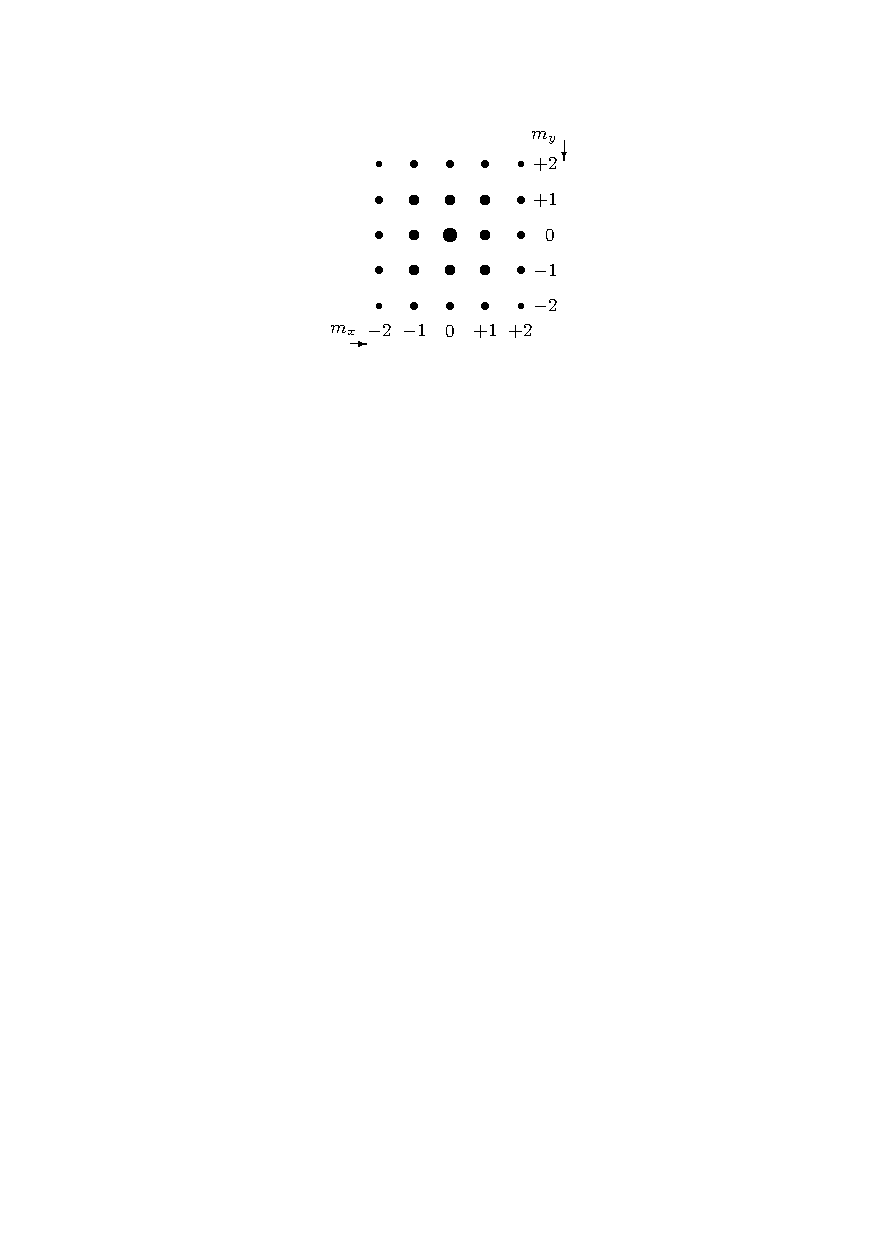
\includegraphics[scale=1.0]{fig1.pdf}}
		\caption{Дифракция Фраунгофера на двумерной решётке (сетке). Максимумы изображены кружками, размеры которых характеризуют интенсивности.}
		\label{fig:max}
	\end{figure}
	
	Если теперь поместить в фокальной плоскости щель так, чтобы через неё проходили дифракционные максимумы с $m_x = 0$ и $m_y =0, \pm 1, \pm 2, ...$ (с $m_y = 0$ и $m_x =0, \pm 1, \pm 2, ...$), то в плоскости $P_2$ получится изображение решётки с горизонтальными (вертикальными) штрихами. Таким образом можно продемонстрировать явление \textit{пространственной фильтрации} -- выделение различных структур в изображении.
	
\newpage

\section*{Экспериментальная установка}
	Схема модели проекционного микроскопа приведена на рис.$\ref{ris:ustanovka}$. Предметом служат сетки, расположенные в кассете. Смена сеток осуществляется поворотом внешнего кольца кассеты.
	
	\begin{figure}[h]
		\center{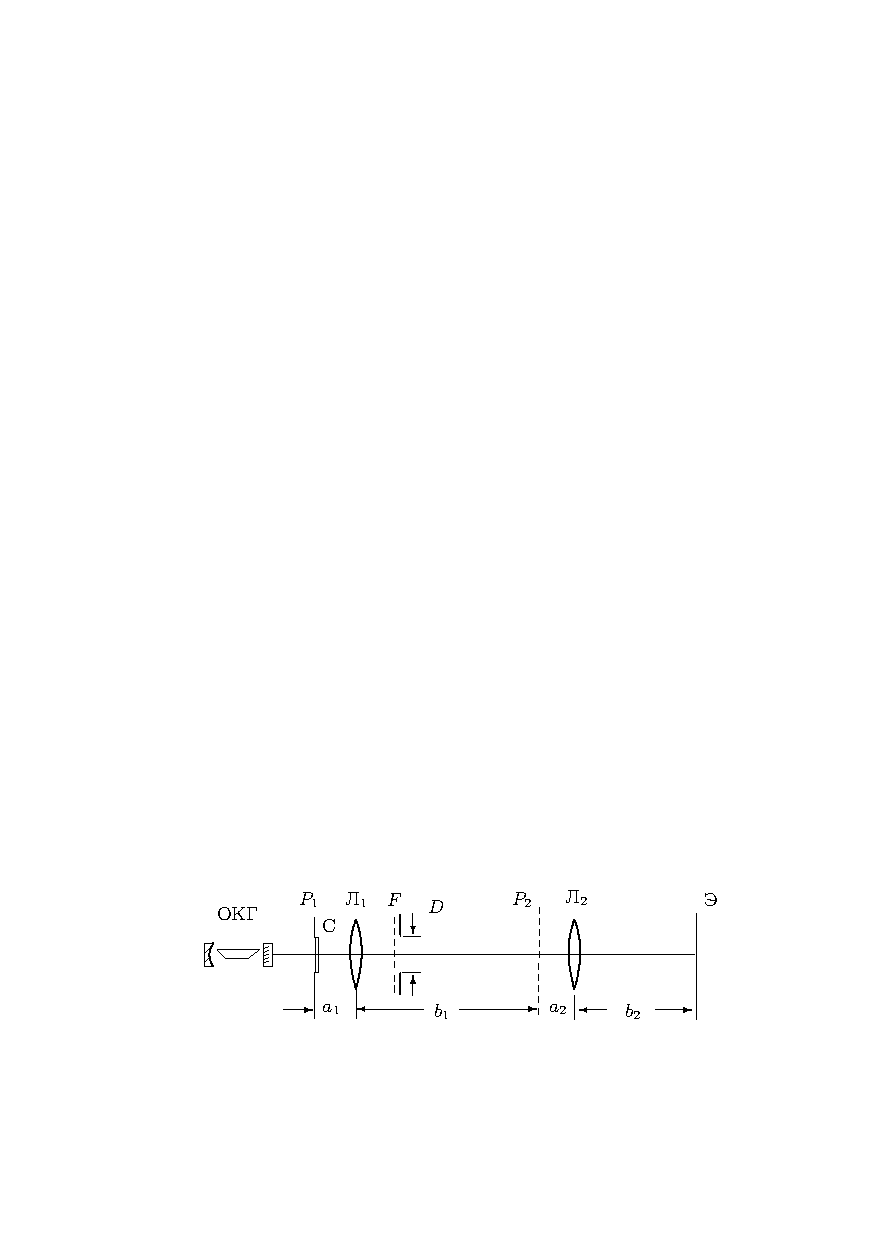
\includegraphics[scale=1.0]{fig2.pdf}}
		\caption{Схема экспериментальной установки.}
		\label{fig:ustanovka}
	\end{figure}
	
	Изображение сетки периодически повторяется -- \textit{репродуцируется} -- в пространстве между сеткой и первой линзой. Для выделения геометрического изображения среди множества репродуцированных изображений сетки на одну из сеток наложена тонкая проволока, то есть непериодический объект, изображение которого не репродуцируется.
	
\section*{Ход работы}

\subsubsection*{Определение периода решеток по их пространственному спектру}

Закрепим касету с двумерными решетками вблизи выходного окна лазера так, чтобы в окошке пол отверстием с сеткой был виден номер сетки.

Вращая наружнее кольцо кассеты, пронаблюдаем на удаленном экране дифракционные картины для разных сеток 

Для определения расстояния между соседними максимумами измерим расстояние между удаленными друг от друга максимумами -- D и число промежутков между ними -- m. Учитывая, что расстояние от сетки до экрана H = 125 мм и углы малые ($\theta \approx \tan \theta = \frac{D}{2m}$, где m -- порядок максимума).Рассчитаем периоды решеток по формуле $\ref{eq:max}$, данные занесем в Таблицу 1 (измерения для каждой из решеток проводились по порядку, начиная с 1)

\begin{table}[h]
\begin{center}
\label{table:spectre}
\caption{Определение периода решеток по их пространственному спектру}
\begin{tabular}{|c|c|c|c|c|}
\hline
\textbf{D, мм} & \textbf{m} & \textbf{D/2, мм} & \textbf{$\theta$} & \textbf{d,mm} \\ \hline
215	$\pm$ 1		& 3          & 107,5            & 0,086                          & 0,019         \\ \hline
190 $\pm$ 1		& 8          & 95               & 0,076                          & 0,056         \\ \hline
200 $\pm$ 1		& 16         & 100              & 0,080                          & 0,106         \\ \hline
46 $\pm$ 1		& 8          & 23               & 0,018                          & 0,231         \\ \hline
62 $\pm$ 1		& 14         & 31               & 0,025                          & 0,300         \\ \hline
\end{tabular}
\end{center}
\end{table} 

где погрешности рассчитывались по формулам:
\begin{gather*}
\sigma_{D} = 1 \ мм \\
%
\sigma_{\theta} = \theta  \frac{\sigma_{D}}{D} \ll \theta \Rightarrow \ погрешность \ пренебрежимо \ мала \\
%
\sigma_{d} = d \frac{\sigma_{\theta}}{\theta} \ll  d \Rightarrow \ погрешность \ пренебрежимо \ мала
\end{gather*}


\newpage

\subsubsection*{Определение периода решеток по изображению, увеличенному с помощью модели микроскопа}

Соберем модель проекционного микроскопа (рис. $\ref{fig:ustanovka}$).Полученные расстояния $a_1 = 130 \ мм \ a_2 = 36 \ мм \ b_1 = 530 \ мм \ b_2 = 630 \ мм$. Тогда определим период решеток по их увеличенному изображению, используя формулы:

\begin{gather*}
\Gamma = \frac{b_1 b_2}{a_1 a_2} = 71,35 \pm 2,06 \\
d = \frac{D}{\Gamma}
\end{gather*}

Результаты занесем в Таблицу 2 (измерения проводились для всех решеток кроме пятой, по порядку, начиная с 1)

\begin{table}[h]
\begin{center}
\caption{Определение периода решеток по изображению}
\label{table:micro}
\begin{tabular}{|c|c|}
\hline
\textbf{D, mm} & \textbf{d, mm} \\ \hline
1,57 $\pm$ 1		& 0,022 $\pm$ 0,01        \\ \hline
3,63 $\pm$ 1		& 0,051 $\pm$ 0,01           \\ \hline
7  $\pm$ 1		& 0,098 $\pm$ 0,03          \\ \hline
10 $\pm$ 1		& 0,140 $\pm$ 0,04         \\ \hline
\end{tabular}
\end{center}
\end{table}

где погрешности рассчитывались по формулам:
\begin{gather*}
\sigma_{a_1} = \sigma_{a_2} = \sigma_{b_1} = \sigma_{b_2} = \sigma_0 = 1 \ мм \\
%
\sigma_{\Gamma} = \Gamma \sqrt{\left(\frac{\sigma_0}{a_1}\right)^2 + \left(\frac{\sigma_0}{a_2}\right)^2 + \left(\frac{\sigma_0}{b_1}\right)^2 + \left(\frac{\sigma_0}{b_2}\right)^2} \\
%
\sigma_{d} = d \sqrt{\left(\frac{\sigma_{\Gamma}}{\Gamma}\right)^2 +  \left(\frac{\sigma_{D}}{D}\right)^2} \approx d \frac{\sigma_{\Gamma}}{\Gamma} 
\end{gather*}

\subsubsection*{Определение периода решёток по оценке разрешающей способности микроскопа}

Поместим щелевую диафрагму в фокальную плоскость линзы $Л_1$ и определим для каждой решетки минимальный размер диафрагмы -- D, при котором на экране еще видно изображение сетки. Данные занесем в Таблицу 3.

\begin{table}[h]
\begin{center}
\caption{Определение периода решёток по оценке разрешающей способности }
\label{table:sposob}
\begin{tabular}{|c|c|}
\hline
\textbf{D, мм} & \textbf{d, мм} \\ \hline
1,45 $\pm$	0,01   & 0,081          \\ \hline
3,25 $\pm$	0,01   & 0,036          \\ \hline
2,06 $\pm$	0,01   & 0,057          \\ \hline
1,18 $\pm$	0,01   & 0,099          \\ \hline
0,93 $\pm$	0,01   & 0,126          \\ \hline
\end{tabular}
\end{center}
\end{table}

где погрешности рассчитывались по формулам:
\begin{gather*}
\sigma_{D} = 0,01 \ мм \\
%
\sigma_{d} = d \frac{\sigma_{D}}{D} \ll d \Rightarrow \ погрешность \ пренебрежимо \ мала
\end{gather*}

\newpage

Для проверки теории Аббе построим график зависимости $d = f(1/D)$, взяв периоды сеток, определенные по спектру. Данные возьмем из Таблицы 1 и Таблицы 3.

	\begin{figure}[h]
		\center{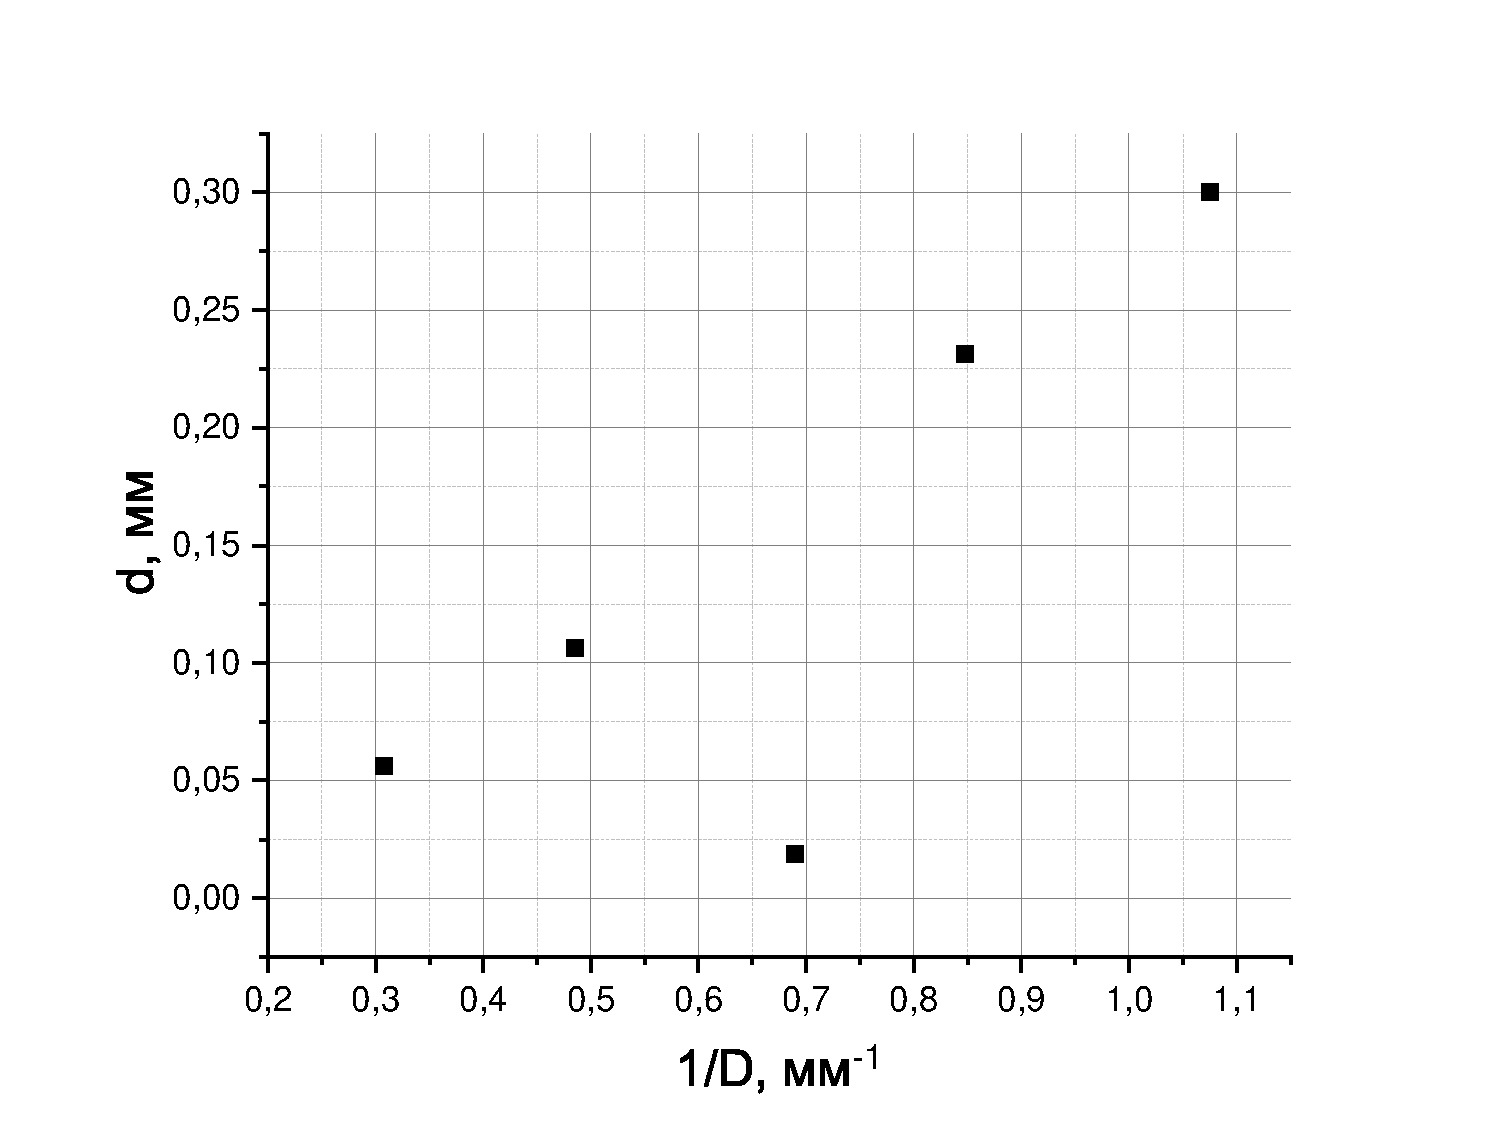
\includegraphics[scale=0.45]{graph1}}
		\caption{Зависимость $d = f(1/D)$ }
		\label{fig:graph1}
	\end{figure}  

Из рис.3 видно, что точка, соответствующая первой дифракционной сетке сильно выпадает из очевидно линейной зависимости. Более того, ее значение более чем в 4 раза отличается от полученного в других опытах. Следовательно, эту точку необходимо исключить. 

	\begin{figure}[h!]
		\center{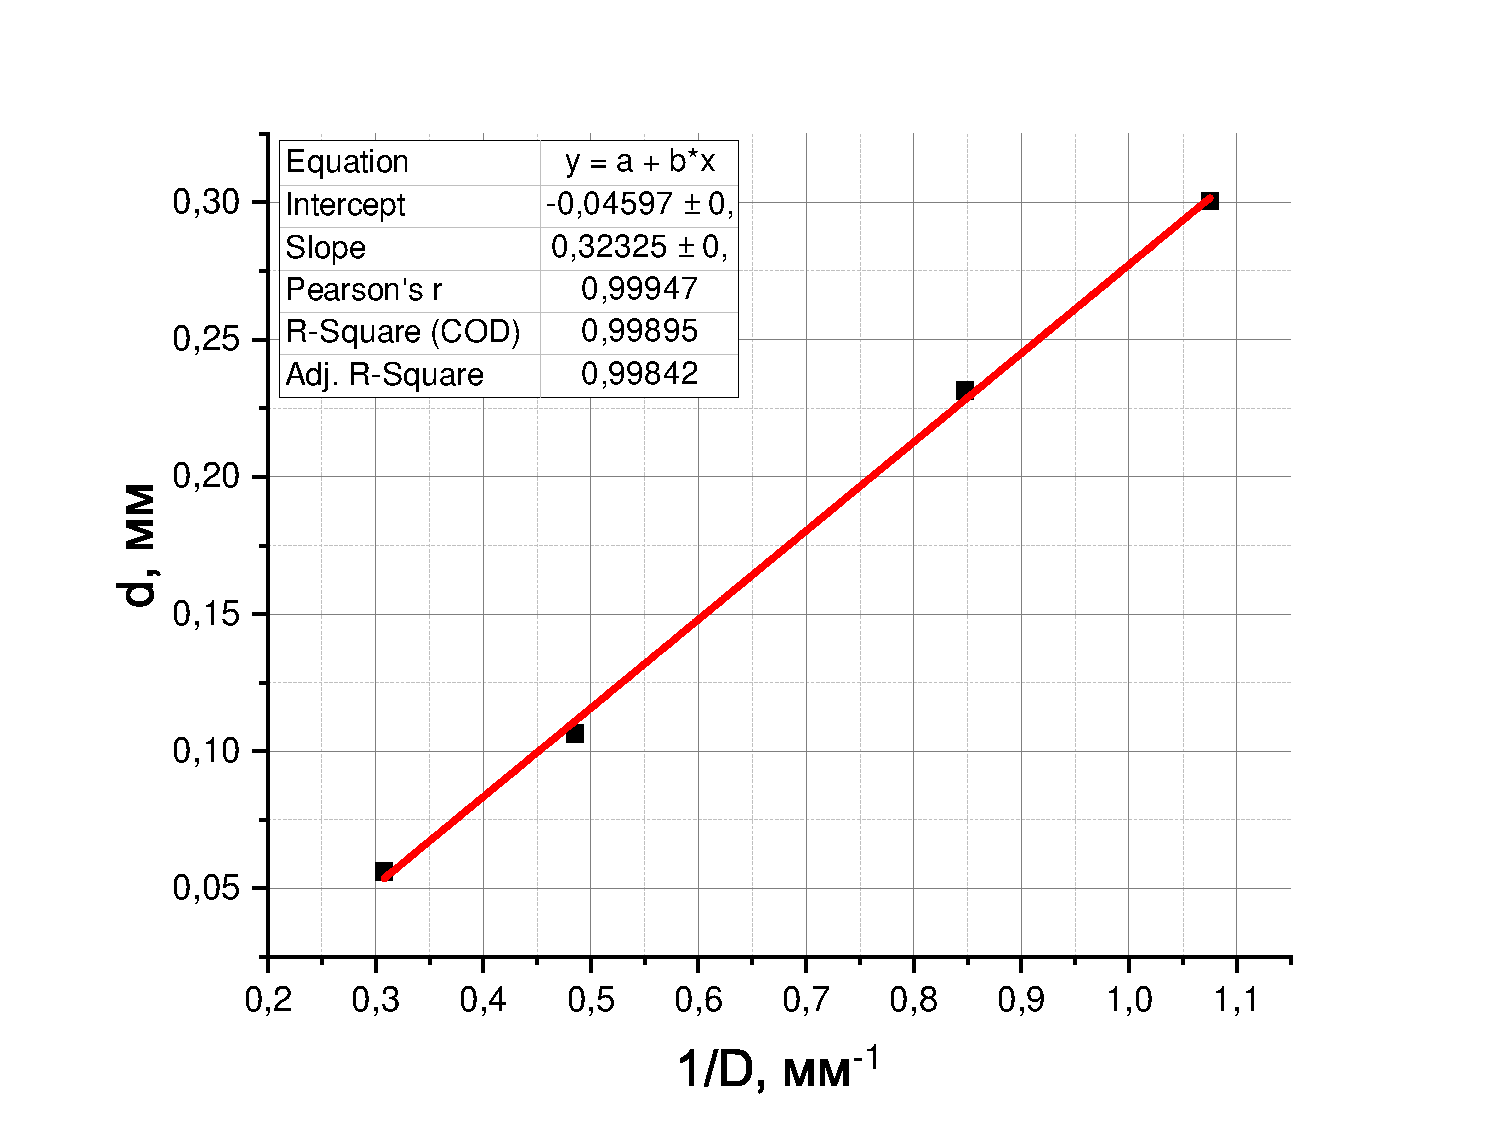
\includegraphics[scale=0.45]{graph2}}
		\caption{Зависимость $d = f(1/D)$ }
		\label{fig:graph2}
	\end{figure}  

\section*{Выводы}
1. Определили периоды дифракционных решеток тремя различными способами \\
2. Экспериментально проверили теорию Аббе





\end{document}